%! suppress = MissingLabel
%! suppress = LineBreak

% CLI args https://tex.stackexchange.com/a/1501
\newif\ifhandout
\input{flags}

%! suppress = MissingLabel
%! suppress = DocumentclassNotInRoot
%! suppress = DiscouragedUseOfDef

% * Make friends tikz & colors
%   https://en.wikibooks.org/wiki/LaTeX/Colors
% * To enable vertical top alignment globally
%   https://tex.stackexchange.com/questions/9889/positioning-content-at-the-top-of-a-beamer-slide-by-default
% * Set handout from CLI
%   https://tex.stackexchange.com/a/1501
\ifhandout
\documentclass[usenames, dvipsnames, handout]{beamer} % https://tex.stackexchange.com/questions/224091/beamer-how-to-disable-pause-temporarily
\else
\documentclass[usenames, dvipsnames]{beamer}
\fi
% ------------------------------------------------

% Graphics
\usepackage{color}
\usepackage{tabularx}
\usepackage{tikz}
% https://tikz.dev/tikz-graphs
\usetikzlibrary{positioning, shapes.geometric, arrows, automata, graphs}
\tikzset{
    expr/.style={ellipse, draw=gray!60, fill=gray!5, very thick, minimum size=7mm, yshift=0.7cm},
    hexpr/.style={ellipse, draw=gray!60, fill=blue!15, very thick, minimum size=7mm, yshift=0.7cm},
    stmt/.style={rectangle, draw=gray!60, fill=gray!5, very thick, minimum size=5mm, yshift=0.7cm},
    decl/.style={rectangle, draw=blue!60, fill=gray!5, very thick, minimum size=5mm, yshift=0.7cm},
    hdecl/.style={rectangle, draw=blue!60, fill=blue!15, very thick, minimum size=5mm, yshift=0.7cm},
    subtree/.style={shape border rotate=90, isosceles triangle, draw=gray!60, fill=gray!5, very thick, minimum size=5mm, yshift=0.0cm},
}
\usepackage{blkarray}
\usepackage{graphicx}
\usepackage{forest} % https://tex.stackexchange.com/questions/198405/how-to-change-the-color-of-subtrees-in-tikz-qtree
% ------------------------------------------------

% Math
\usepackage{amsmath, amsfonts}
\usepackage{amssymb}
\usepackage{proof}
\usepackage{mathrsfs}
% Crossed-out symbols
% https://tex.stackexchange.com/questions/75525/how-to-write-crossed-out-math-in-latex
\usepackage[makeroom]{cancel}
\usepackage{mathtools}
% ------------------------------------------------

% Additional font sizes
% https://www.overleaf.com/learn/latex/Questions/How_do_I_adjust_the_font_size%3F
\usepackage{moresize}
% Additional colors
% https://www.overleaf.com/learn/latex/Using_colours_in_LaTeX
\usepackage{xcolor}
% Textual math symbols
\usepackage{textcomp}
% ------------------------------------------------

% Language
\usepackage[utf8] {inputenc}
\usepackage[T2A] {fontenc}
\usepackage[english, russian] {babel}
\usepackage{indentfirst, verbatim}
\usetikzlibrary{cd, babel}
% ------------------------------------------------

% Fonts: https://sites.math.washington.edu/~reu/docs/latex_symbols.pdf
\usepackage{stmaryrd}
\usepackage{cmbright}
\usepackage{wasysym}
\usepackage[weather]{ifsym} % https://tex.stackexchange.com/questions/100424/how-to-use-the-ifsym-package
% https://tex.stackexchange.com/questions/615300/pdflatex-builtin-glyph-names-is-empty
\pdfmapline{=dictsym DictSym <dictsym.pfb}
\pdfmapline{=pigpen <pigpen.pfa}
\usepackage{dictsym}
% ------------------------------------------------

% Code
% * Needs -shell-escape build flag
%   https://tex.stackexchange.com/questions/99475/how-to-invoke-latex-with-the-shell-escape-flag-in-texstudio-former-texmakerx
% * Set build directory
%   https://tex.stackexchange.com/questions/339931/latex-minted-package-using-custom-output-directory-build
\usepackage{minted}
\setminted{xleftmargin=\parindent, autogobble, escapeinside=\#\#}
% ------------------------------------------------

% Template
\usetheme{CambridgeUS}
\usecolortheme{dolphin}
% https://tex.stackexchange.com/questions/231439/beamer-how-to-make-font-larger-for-page-numbers
\setbeamerfont{headline}{size=\scriptsize}
\setbeamerfont{footline}{size=\scriptsize}
% Remove heddline
% https://tex.stackexchange.com/questions/33146/how-could-i-remove-a-header-in-a-beamer-presentation
%\setbeamertemplate{headline}{}
% Slide sizes
% https://tex.stackexchange.com/questions/56768/how-to-set-a-small-default-font-size-with-beamer
%\geometry{paperwidth=140mm,paperheight=105mm} % 4:3
\geometry{paperwidth=168mm,paperheight=105mm} % 16:10
% Remove navigation bar
% https://stackoverflow.com/questions/3210205/how-to-get-rid-of-navigation-bars-in-beamer
\beamertemplatenavigationsymbolsempty
% ------------------------------------------------

% Bullets
% https://9to5science.com/change-bullet-style-formatting-in-beamer
% https://tex.stackexchange.com/questions/185742/i-need-to-change-color-of-beamer-itemize-and-subitem-separately
\setbeamertemplate{itemize item}{\scriptsize\raise1.25pt\hbox{\donotcoloroutermaths$\blacktriangleright$}}
\setbeamertemplate{itemize subitem}{\scriptsize\raise1.5pt\hbox{\donotcoloroutermaths$\blacktriangleright$}}
\setbeamertemplate{itemize subsubitem}{\tiny\raise1.5pt\hbox{\donotcoloroutermaths$\blacktriangleright$}}
\setbeamertemplate{enumerate item}{\insertenumlabel.}
\setbeamertemplate{enumerate subitem}{\insertenumlabel.\insertsubenumlabel}
\setbeamertemplate{enumerate subsubitem}{\insertenumlabel.\insertsubenumlabel.\insertsubsubenumlabel}
% ------------------------------------------------

% Table of contents format
% https://tex.stackexchange.com/questions/642927/format-table-of-contents-in-beamer
\setbeamertemplate{section in toc}{%
        {\color{blue}\inserttocsectionnumber.}
    \inserttocsection\par%
}
\setbeamertemplate{subsection in toc}{%
        {\color{blue}\hspace{1em}\scriptsize\raise1.25pt\hbox{\donotcoloroutermaths$\blacktriangleright$}}
    \inserttocsubsection\par%
}
\setbeamertemplate{subsubsection in toc}{%
        {\color{blue}\hspace{2em}\tiny\raise1.25pt\hbox{\donotcoloroutermaths$\blacktriangleright$}}
    \inserttocsubsubsection\par%
}
% ------------------------------------------------

% Misc
\usepackage{multicol}
\usepackage{hyperref}
\usepackage{soul} % https://tex.stackexchange.com/questions/23711/strikethrough-text
% ------------------------------------------------

% Fix \pause for amsmath package envs (black black magic)
% https://tex.stackexchange.com/questions/16186/equation-numbering-problems-in-amsmath-environments-with-pause/75550#75550
% https://tex.stackexchange.com/questions/6348/problem-with-beamers-pause-in-alignments
%! suppress = Makeatletter
\makeatletter
\let\save@measuring@true\measuring@true
\def\measuring@true{%
    \save@measuring@true
    \def\beamer@sortzero##1{\beamer@ifnextcharospec{\beamer@sortzeroread{##1}}{}}%
    \def\beamer@sortzeroread##1<##2>{}%
    \def\beamer@finalnospec{}%
}
%! suppress = Makeatletter
\makeatother
% ------------------------------------------------

% Sections
\newcommand{\sectionplan}[1]{\section{#1}%
    \begin{frame}[noframenumbering]{Содержание}
        \tableofcontents[currentsection]
    \end{frame}
}
\newcommand{\subsectionplan}[1]{\subsection{#1}%
    \begin{frame}[noframenumbering]{Содержание}
        \tableofcontents[currentsubsection]
    \end{frame}
}
% ------------------------------------------------

% Footnotes
\renewcommand{\thefootnote}{\arabic{footnote}}
\renewcommand{\thempfootnote}{\arabic{mpfootnote}}
% https://tex.stackexchange.com/questions/28465/multiple-footnotes-at-one-point
\usepackage{fnpct}
% ------------------------------------------------

% Links
% Colors also links on slide foot.
%\hypersetup{
%    colorlinks=true,
%    citecolor=blue,
%    linkcolor=blue,
%    urlcolor=blue
%}
% ------------------------------------------------

% Appendix
% Slide numbers
% https://tex.stackexchange.com/questions/70448/dont-count-backup-slides
\usepackage{appendixnumberbeamer}
\newcommand{\backupbegin}{
    \newcounter{framenumbervorappendix}
    \setcounter{framenumbervorappendix}{\value{framenumber}}
}
\newcommand{\backupend}{
    \addtocounter{framenumbervorappendix}{-\value{framenumber}}
    \addtocounter{framenumber}{\value{framenumbervorappendix}}
}
% ------------------------------------------------

% Custom commands
% * Decor
\newcommand{\newtopic}[0]{$+$} % item: new topic on "in previous series"
\newcommand{\then}{$\Rightarrow$} % item: consequences
\newcommand{\pop}[0]{\SunCloud} %item:  general eduation
\newcommand{\popslide}[0]{(\pop)}
\newcommand{\advanced}[0]{$\varhexstar$} % item: advanced science
\newcommand{\advancedslide}[0]{(\advanced)}
\newcommand{\practical}[0]{\dstechnical} % item: practical programming notions
\newcommand{\practicalslide}[0]{(\practical)}
\newcommand{\todo}[0]{todo} % item: question
\newcommand{\answer}[0]{\Lightning} % item: answer to the previous question
\newcommand{\eg}[0]{e.g.} % item: example
\newcommand{\defi}[0]{$\Delta$} % item: definition on smth
\newcommand{\textdefi}[1]{\textbf{#1}}
\newcommand{\positive}{$+$} % item: pros
\newcommand{\negative}{{\color{red} $-$}} % item: cons
\newcommand%! suppress = EscapeHashOutsideCommand
\NB[1][0.3]{N\kern-#1em{B}} % default kern amount: -0.3em
\renewcommand{\emph}[1]{{\color{blue} \textit{#1}}}
\newcommand{\vocab}[1]{\textbf{#1}} % item: important new word
% * Lambda calculi
\newcommand{\comb}[1]{\mathbf{#1}} % defined combinator
\newcommand{\term}[1]{\mathbf{#1}} % predefined lambda-term reference
\newcommand{\termdef}{\coloneqq} % lamda term binding
\newcommand{\step}{\rightsquigarrow} % reduction step
\newcommand{\sstep}{\twoheadrightarrow} % multiple steps reduction
\newcommand{\ap}{~} % lambda-term application
\newcommand{\subst}[3]{\left[#2 \mapsto #3 \right] #1} % substitution
\newcommand{\eqbeta}{=_\beta} % beta equality
\newcommand{\eqeta}{=_\eta} % eta-equality
\newcommand{\eqt}{=} % tree-equality of terms
\newcommand{\tlist}[1]{\term{[}#1\term{]}} % list-term
% * Legacy
%\newcommand{\err}[0]{\textcolor{red}{ошибка}} % compilation error

% ------------------------------------------------

% Speaker notes
% https://tex.stackexchange.com/questions/114219/add-notes-to-latex-beamer
% https://tex.stackexchange.com/questions/35444/split-beamer-notes-across-multiple-notes-pages/35496#35496
%\setbeameroption{show notes on second screen=right} % enable speaker notes
%--------------------------------------

\author[]{Андрей Стоян, Илья Колегов, Дмитрий Халанский}
\institute[MSE ITMO]{MSE ITMO}


\title[Типы в $\lambda$-исчислении]{Практика 3. Типы в $\lambda$-исчислении}
\date{осень 2024}

\begin{document}

    \setcounter{framenumber}{-1}
    \maketitle

    \begin{frame}{В предыдущих сериях}
        \begin{itemize}
            \item Синтаксис и семантика лямбда-исчисления
            \item Эквивалентности на термах
            \item[\newtopic] Синтаксис типов и термов $\lambda_\to$
            \item[\newtopic] Правила типизации $\lambda_\to$
            \item[\newtopic] Гарантии системы $\lambda_\to$
        \end{itemize}
    \end{frame}

    \begin{frame}[noframenumbering]{Содержание}
        \tableofcontents
    \end{frame}


    \sectionplan{Идея систем типов}

    \begin{frame}{Мотивация статического анализа программ}
        \begin{itemize}
            \item Программное обеспечение — это сложно
            \item В программах случаются ошибки (постоянно и неизбежно)
            \item Поиск ошибок может занимать годы, десятилетия, вечность
            \item Нужны методы для того, чтобы судить о программах и их
            свойствах автоматически
            \item Программы могут работать долго
            \item Хотим отвергать ``плохие'' программы до исполнения (статически)
        \end{itemize}
    \end{frame}

    \begin{frame}{Анализ типов}
        \vspace{-0.5em}
        \begin{block}{Идея анализа типов}
            \begin{itemize}
                \item Попытаемся приписать каждой ноде программы синтаксические метки по определённым правилам
                \item Если метки таким образом приписать можно --- программа ``хорошая''
                \item Вид таких меток и правил задаётся \textit{системой типов}
                \item Анализ типов --- разновидность статического анализа ($\subset$ constraint-based analysis)
            \end{itemize}
        \end{block}
        \pause
        \vspace{-3em}
        \begin{columns}[onlytextwidth]
            \begin{column}[t]{0.15\textwidth}
                \begin{center}
                    \begin{tikzpicture}
                        \node [decl] (f) {$f : int \to int$};
                        \node [expr] (lam) [below=of f] {$\lambda : int \to int$};
                        \node [decl] (y) [below right = of lam] {$y {\color{red}~: int}$};
                        \node [expr] (div) [below=of lam] {$\div : int$};
                        \node [expr] (x) [below left=of div] {$x : int$};
                        \node [expr] (plus) [below right = of div] {$+ : int$};
                        \node [expr] (param) [below left=of plus] {$y : int$};
                        \node [expr] (two) [below right = of plus] {$2 : int$};
                        \draw[->] (lam) -- (f);
                        \draw[->] (div) -- (lam);
                        \draw[->] (plus) -- (div);
                        \draw[->] (x) -- (div);
                        \draw[->] (two) -- (plus);
                        \draw[->] (param) -- (plus);
                        \draw[->] (y) -- (lam);
                    \end{tikzpicture}
                \end{center}
            \end{column}\hfill%
            \pause%
            \begin{column}[t]{0.62\textwidth}
                \begin{center}
                    \begin{tikzpicture}
                        \node [expr] (app) {$@ : int$};
                        \node [expr] (f) [below left =of app] {$f : int \to int$};
                        \node [expr] (mult) [below right= of app] {$\div : int$};
                        \node [expr] (ten) [below left= of mult] {$10 : int$};
                        \node [expr] (four) [below right= of mult] {$4 : int$};
                        \draw[->] (mult) -- (app);
                        \draw[->] (f) -- (app);
                        \draw[->] (ten) -- (mult);
                        \draw[->] (four) -- (mult);
                    \end{tikzpicture}
                \end{center}
            \end{column}
        \end{columns}
    \end{frame}

    \begin{frame}[fragile]{Роль типов в ЯП}
        \begin{itemize}
            \item Выявление некоторых классов ошибок
            \begin{minted}{haskell}
                GHCi> length 42         -- Ошибка: на вход не список, а число
                GHCi> foldr (+) "ABCDE" -- Ошибка: плюс работает на числах, но не символах
            \end{minted}
            \item Механизм абстракции: интерфейс\footnote{В общем смысле, не мешать с ООП.}, скрывающий детали реализации
            \item Документация --- как использовать сущность
            \item Обеспечивают безопасность языка --- нет сегфолтов
            \item \textit{Частичная} спецификация поведения сущности
            \item Эффективность --- можно производить более агрессивные оптимизации
        \end{itemize}
    \end{frame}

    \begin{frame}{Ограниченность систем типов \popslide}
        \begin{itemize}
            \item Хотелось бы, чтобы все ``хорошие'' программы типизировались, а все ``плохие'' ~--- нет
            \item Однако по теореме Успенского-Райса задача проверки любого нетривиального\footnote{Существуют программы, как обладающие таким свойством, так и не обладающие.} свойства программы неразрешима
        \end{itemize}
        \pause
        \vspace{1em}
        В чем подвох с системами типов? \pause
        \begin{itemize}
            \item Всё, что типизируется, --- ``хорошее'', но обратное не всегда верно
            \item[$\Rightarrow$] Всегда существуют ``хорошие'' программы, которые не типизируются\footnote{В маргинальных случаях (e.g. TypeScript) к тому же существуют ``плохие'', которые типизируются.}
        \end{itemize}
        \begin{center}
            
\includegraphics[height=0.25\textheight]{figs/types}
        \end{center}
    \end{frame}

    \begin{frame}{При чём тут ФП? \popslide}
        \begin{itemize}
            \item Парадигме агрессивного абстрагирования требуются гибкие системы типов
            \item ФП языки минималистичные и регулярные --- с ними проще работать
        \end{itemize}
        \begin{center}
            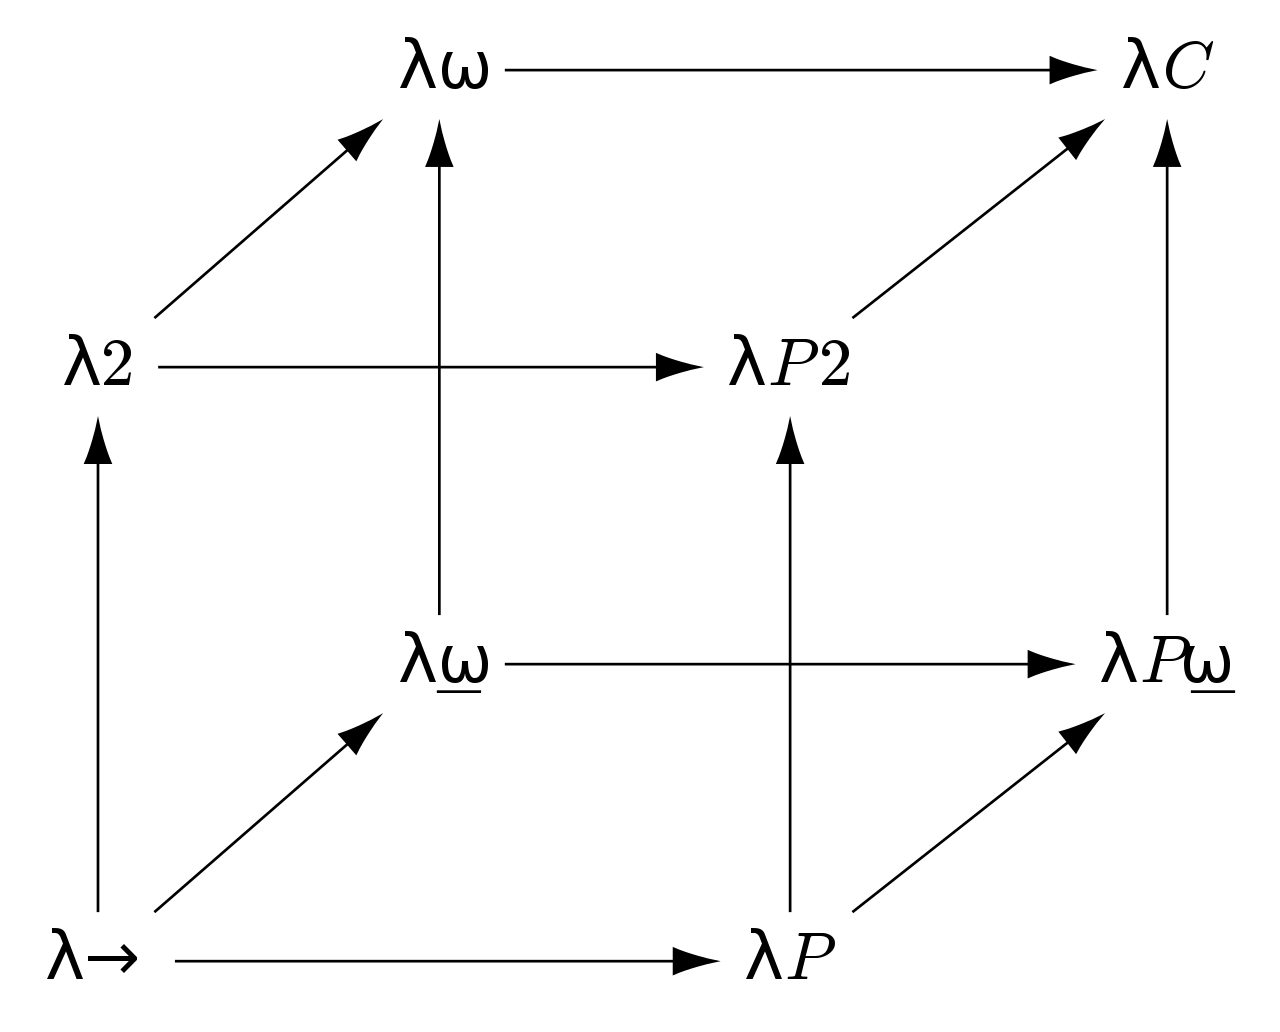
\includegraphics[height=0.6\textheight]{figs/cube}
        \end{center}
    \end{frame}


    \sectionplan{Контекст типизации}

    \begin{frame}[fragile]{Контекст типизации}
        \begin{itemize}
            \item \pause В программах используются введённые ранее имена
            \item \pause Для типизации нужно знать типы сущностей, связанных ранее с этими именами
            \item \pause Будем поддерживать доп. структуру данных, которую будем заполнять именами с соответствующими им типами в процессе обхода дерева программы
        \end{itemize}
        \pause
        \begin{block}{Пример на Си}
            \vspace{-1em}
            \begin{columns}[onlytextwidth]
                \begin{column}{0.485\textwidth}
                    \begin{minted}{c}
                    int dostrange(int a, char i) {
                        // point 0
                        int c = 5;
                        for (int i = 0; i < 15; ++i) {
                            i -= 1; // point 1
                            long r = i;
                            i *= r; // point 2
                        }
                        return a + (int)i * c; // point 3
                    }
                    \end{minted}
                \end{column}\hfill%
                \begin{column}{0.485\textwidth}
                    Контекст типизации в каждой из точек:
                    \begin{enumerate}
                        \setcounter{enumi}{-1}
                        \item $\{a : \mathrm{int},\, i : \mathrm{char}\}$
                        \item \pause $\{a : \mathrm{int},\, c : \mathrm{int},\, i : \mathrm{int}\}$
                        \item \pause $\{a : \mathrm{int},\, c : \mathrm{int},\, i : \mathrm{int},\, r : \mathrm{long}\}$
                        \item \pause $\{a : \mathrm{int},\, c : \mathrm{int},\, i : \mathrm{char}\}$
                        \item[$+$] \pause Глобальные определения: \pause \texttt{<}, \texttt{+}, \texttt{*}\ldots
                    \end{enumerate}
                \end{column}
            \end{columns}
        \end{block}
    \end{frame}

    \begin{frame}{Контекст типизации: пример на лямбда-исчислении}
        В чистом лямбда-исчислении имена вводятся с помощью абстракции.
        \begin{columns}[onlytextwidth]
            \begin{column}{0.485\textwidth}
                \begin{center}
                    \begin{tikzpicture}
                        \node [expr] (lamf) {(0) $\lambda$};
                        \node [decl] (f) [below right=of lamf] {$f {\color{red}~: \tau}$};
                        \node [expr] (lamg) [below  =of lamf] {(1) $\lambda$};
                        \node [decl] (g) [below right= of lamg] {$g {\color{red}~: \sigma}$};
                        \node [expr] (lamx) [below  =of lamg] {(2) $\lambda$};
                        \node [decl] (x) [below right= of lamx] {$x {\color{red}~: \zeta}$};
                        \node [expr] (apf) [below  =of lamx] {$@$};
                        \node [expr] (vf) [below left= of apf] {$f$};
                        \node [expr] (apg) [below right=of apf] {$@$};
                        \node [expr] (vg) [below left= of apg] {$g$};
                        \node [expr] (vx) [below right= of apg] {$x$};
                        \draw[->] (lamg) -- (lamf);
                        \draw[->] (lamx) -- (lamg);
                        \draw[->] (f) -- (lamf);
                        \draw[->] (g) -- (lamg);
                        \draw[->] (x) -- (lamx);
                        \draw[->] (apf) -- (lamx);
                        \draw[->] (apg) -- (apf);
                        \draw[->] (vf) -- (apf);
                        \draw[->] (vg) -- (apg);
                        \draw[->] (vx) -- (apg);
                    \end{tikzpicture}
                \end{center}
            \end{column}\hfill%
            \begin{column}{0.485\textwidth}
                Контекст типизации для каждой вершины:
                \begin{enumerate}
                    \setcounter{enumi}{-1}
                    \item \pause $\emptyset$
                    \item \pause $\{f : \tau\}$
                    \item \pause $\{f : \tau, g : \sigma\}$
                    \item[$*.$] \pause $\{f : \tau, g : \sigma, x : \zeta\}$
                \end{enumerate}
            \end{column}
        \end{columns}
    \end{frame}


    \sectionplan{STLC / simply typed $\lambda$-calculus / $\lambda_\to$}

    \begin{frame}[fragile]{STLC типизация интуитивно}
        \begin{itemize}
            \item[\todo] Припишите тип терму $\lambda x^{\alpha}\ldotp x$
            \item[\answer] \pause
            \begin{itemize}
                \item Терм задаёт функцию --- тип стрелочный: $\alpha \to ~?$
                \item Типизируем тело, зная $\Gamma = \{x : \alpha\}$, $\lambda x^\alpha\ldotp \underbrace{x}$
                \item % todo
            \end{itemize}
            \item[\todo] Припишите тип терму $\lambda x^\alpha~f^{\alpha \to \beta}\ldotp f \ap x$
            \item[\answer] \pause % todo
            \item[\todo] Припишите тип терму $\lambda x~y\ldotp x$
            \item[\answer] % todo
            \item[\todo] Припишите тип терму $\lambda x~y~f\ldotp f \ap x \ap y$ % todo
            \item[\answer] % todo
        \end{itemize}
    \end{frame}

    \begin{frame}[fragile]{STLC население типов интуитивно}
        \begin{itemize}
            \item[\todo] Населите тип $(\beta\to\gamma)\to(\alpha\to\beta)\to\alpha\to\gamma$
            \item[\answer] \pause % todo
        \end{itemize}
    \end{frame}

    % todo переместить контекст типизации сюда

    \begin{frame}{Определение \secname}
        \vspace{-0.5em}
        \pause
        \begin{block}{Синтаксис типов в $\lambda_{\rightarrow}$}
            \begin{description}
                \item[Типовые переменные] \vspace{-1em} $\alpha, \beta, \ldots \in \mathbb{T}$
                \hspace{2em}
                \begin{tikzpicture}
                    \node [expr] (a) {$\alpha$};
                \end{tikzpicture}
                \item[Стрелочные типы] \vspace{-2em} $\sigma, \tau \in \mathbb{T} \Rightarrow (\sigma\rightarrow\tau)\in\mathbb{T}$\footnote{Стрелочка --- правоассоциативный оператор: $\tau \to (\sigma \to \zeta) \eqt \tau \to \sigma \to \zeta$.}
                \hspace{2em}
                \begin{tikzpicture}
                    \node [expr] (arr) {$\to$};
                    \node [subtree] (t) [below left= of arr] {$\sigma$};
                    \node [subtree] (s) [below right= of arr] {$\tau$};
                    \draw[->] (t.north) -- (arr);
                    \draw[->] (s.north) -- (arr);
                \end{tikzpicture}
            \end{description}
        \end{block}
        \pause
        \begin{block}{Утверждение типизации}
            \begin{itemize}
                \item Синтаксис: $\Gamma$ --- контекст, $M \in \Lambda, \sigma \in \mathbb{T}$, то $\Gamma \vdash M : \sigma$ --- утверждение типизации
                \item Синтаксическая категория, увязывающая вместе термы и типы с контекстом
                \item Утверждает, что в контексте $\Gamma$ терм $M$ имеет тип $\sigma$
            \end{itemize}
        \end{block}
        \pause
        \begin{block}{Правила вывода утверждений типизации в $\lambda_{\rightarrow}$}
            \vspace{-1em}
            \begin{center}
                \[
                    \begin{array}{l c r}
                        \infer[ctx]{\Gamma \vdash x: \sigma}{(x: \sigma) \in \Gamma}
                        &
                        \infer[elim\to]{\Gamma \vdash M\;N : \tau}{\Gamma \vdash M : \sigma \to \tau & \Gamma \vdash N : \sigma}
                        &
                        \infer[intro\to]{\Gamma \vdash \lambda x^{\color{red} \sigma}\ldotp M : \sigma \to \tau}{\{x : \sigma\} \cup \Gamma \vdash M : \tau}
                    \end{array}
                \]
            \end{center}
        \end{block}
    \end{frame}

    \subsectionplan{Задача проверки типа}

    \begin{frame}{Проверка типа комбинатора $\term{B}$ в $\lambda_\to$}
        \begin{block}{Правила вывода утверждений типизации в $\lambda_{\rightarrow}$}
            \vspace{-1em}
            \begin{center}
                \[
                    \begin{array}{l c r}
                        \infer[ctx]{\Gamma \vdash x: \sigma}{(x: \sigma) \in \Gamma}
                        &
                        \infer[elim\to]{\Gamma \vdash M\;N : \tau}{\Gamma \vdash M : \sigma \to \tau & \Gamma \vdash N : \sigma}
                        &
                        \infer[intro\to]{\Gamma \vdash \lambda x^{\color{red} \sigma}\ldotp M : \sigma \to \tau}{\{x : \sigma\} \cup \Gamma \vdash M : \tau}
                    \end{array}
                \]
            \end{center}
        \end{block}
        \pause
        %! suppress = EscapeAmpersand
        \[\resizebox{0.8\hsize}{!}{
            \infer[\visible<3->{intro\to}]
            {\emptyset \vdash \lambda f~g~x.~f~(g~x) : (\beta \to \gamma) \to (\alpha \to \beta) \to \alpha \to \gamma}
            {\visible<3->{
                \infer[\visible<4->{intro\to}]
                {\{f: \beta \to \gamma\} \vdash \lambda g~x.~f~(g~x) : (\alpha \to \beta) \to \alpha \to \gamma}
                {\visible<4->{
                    \infer[\visible<5->{intro\to}]
                    {\{f : \beta \to \gamma, g : \alpha \to \beta\} \vdash \lambda x.~f~(g~x) : \alpha \to \gamma}
                    {\visible<5->{
                        \infer[\visible<6->{elim\to}]{\{f : \beta \to \gamma, g : \alpha \to \beta, x:  \alpha\} \vdash f~(g~x) : \gamma}
                        {\visible<6->{
                            \infer[\visible<7->{ctx}]{\Gamma \vdash f : \beta \to \gamma}{} &
                            \infer[\visible<8->{elim\to}]{\Gamma \vdash g~x : \beta}{\visible<8->{
                                \infer[\visible<9->{ctx}]{\Gamma \vdash g : \alpha \to \beta}{} &
                                \infer[\visible<10->{ctx}]{\Gamma \vdash x : \alpha}{}
                            }}
                        }}
                    }}
                }}
            }}
        }\]
        \begin{itemize}
            \item \visible<11->{Получилось перевёрнутое синтаксическое дерево терма!}
            \item[\todo] \visible<12->{Меняется ли что-то для типизации в стиле Чёрча?}
            \item[\answer] \visible<13->{В этой задаче --- нет: тип терму уже приписан, информации для построения дерева достаточно}
        \end{itemize}
    \end{frame}

    \begin{frame}[noframenumbering]{Таинственные связи \popslide}
        Дерево вывода типа комбинатора $\term{B}$ или \visible<2->{вывод силлогизма в исчислении высказываний?}
        %! suppress = EscapeAmpersand
        \[\resizebox{0.8\hsize}{!}{
            \infer[intro\to]{\emptyset \vdash \visible<1>{{\color{blue} \lambda f~g~x.~f~(g~x) :~}} (\beta \to \gamma) \to ({ \alpha} \to \beta) \to \alpha \to \gamma}{
                \infer[intro\to]{\{\visible<1>{{\color{blue}f:~}} \beta \to \gamma\} \vdash \visible<1>{{\color{blue} \lambda g~x.~f~(g~x) :~}} ({ \alpha} \to \beta) \to \alpha \to \gamma}{
                    \infer[intro\to]{\{\visible<1>{{\color{blue}f:~}} \beta \to \gamma, \visible<1>{{\color{blue}g:~}} {\alpha} \to \beta\} \vdash \visible<1>{{\color{blue} \lambda x.~f~(g~x) :~}} \alpha \to \gamma }{
                        \infer[MP]{\{\visible<1>{{\color{blue}f:~}} \beta \to \gamma, \visible<1>{{\color{blue}g:~}} {\alpha} \to \beta, \visible<1>{{\color{blue}x:~}}  \alpha\} \vdash \visible<1>{{\color{blue} f~(g~x) :~}} \gamma }{
                            \infer[InCtx]{\Gamma \vdash \visible<1>{{\color{blue} f :~}} \beta \to \gamma}{} &
                            \infer[MP]{\Gamma \vdash \visible<1>{{\color{blue} g~x :~}} \beta}{
                                \infer[InCtx]{\Gamma \vdash \visible<1>{{\color{blue} g :~}} {\alpha} \to \beta}{} &
                                \infer[InCtx]{\color{black} \Gamma \vdash \visible<1>{{\color{blue} x :~}} { \alpha}}{}
                            }}}}
            }
        }\]
    \end{frame}

    \subsectionplan{Задача населения типа}

    \begin{frame}{Простые примеры задач населения}
        % todo убрать смущение долой
        Найдите все возможные варианты для терма $M$ в каждом из случаев:
        \begin{enumerate}
            \item $\{x: \beta\} \vdash M: \alpha \to \alpha$
            \item $\{x: \beta\} \vdash M: \alpha \to \beta$
            \item $\{x: \beta\} \vdash M: \alpha \to \gamma$
        \end{enumerate}
        \pause
        \vspace{0.5em}
        Решение:
        \begin{enumerate}
            \item \pause $M \eqt \lambda y\ldotp y$
            \begin{itemize}
                \item На вход вызывающий может подать что угодно
                \item На выходе обязан ожидать, что $M$ вернёт значение того же типа, что подаётся на вход
            \end{itemize}
            \item \pause $M \eqt \lambda y\ldotp x$
            \begin{itemize}
                \item На вход вызывающий может подать что угодно
                \item На выходе обязан ожидать значение того же типа, что имеет $x$
            \end{itemize}
            \item \pause Таких $M$ не может быть
            \begin{itemize}
                \item На вход вызывающий может подать что угодно
                \item На выходе может требовать что угодно
            \end{itemize}
        \end{enumerate}
    \end{frame}

\end{document}
